\documentclass[11pt, oneside]{turabian-thesis} 
\usepackage{turabian-formatting}
\usepackage[authoryear]{natbib}
\fancypagestyle{plain}{\pagestyle{fancy}}

\usepackage{graphicx}
\usepackage[percent]{overpic}
\usepackage{booktabs,siunitx}
\usepackage{caption}
\usepackage{subcaption}
\usepackage{amssymb}
\usepackage{amsmath}
\usepackage{multirow}
\usepackage{rotating}
\usepackage{url}
\usepackage{amsmath}
\usepackage{amsthm}
\usepackage{placeins}
\usepackage[usenames,dvipsnames,svgnames,table]{xcolor}
\usepackage{todonotes}
\usepackage{tikz}
\usetikzlibrary{positioning}
\usepackage[super]{nth}

\definecolor{lightblue}{rgb}{0.93,0.95,1.0}
\definecolor{lightgray}{gray}{0.9}



\begin{document}
\pagenumbering{gobble}
\tableofcontents
\listoffigures
\listoftables


\chapter{Introduction} \label{chpt:intro}
\pagenumbering{arabic}

This is the first chapter. In it I can reference a figure (\ref{fig:figureLabel}). I can also create a subsection and reference a table.
\begin{figure}[htbp] %  figure placement: here, top, bottom, or page
   \centering
   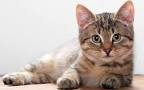
\includegraphics[scale=.75]{cat.jpg} 
   \caption{This is a picture of a cat.}
   \label{fig:figureLabel}
\end{figure}

\FloatBarrier
\subsection{I am a subsection} \label{chpt:subsection}
I can put in a float barrier to make sure that Table \ref{tbl:CSperf} appears in this subsection and does not migrate above.\\ %Without the newline marker the table appears very close to the end of the text. This is purely aesthetic so feel free to disagree.

\begin{table}[h!] \scriptsize %tables can be different sizes
\caption{Index of fruit belonging to people.} %End title with a period!!
\begin{center}
\rowcolors{1}{}{lightblue}
\begin{tabular}{ l c c c }
	\toprule
		\textbf{Name} & \textbf{Apples} \textbf{Oranges} & \textbf{Peaches}\\
		\cmidrule(r){1 - 4}
	Mike & 10 & 34 & 2\\
	John & 2 & 23 & 32\\
	Paul & 4 & 45 & 34\\
	Sam & 34 & 3 & 23\\
	\bottomrule
\end{tabular}
\end{center}
\footnotesize{This is where the explanation of the table goes.}
\label{tbl:CSperf}
\end{table}

You can add math as well:
\begin{align}
	ax + by &= c.
\end{align}
This can be done in whatever way you would normally add mathematic symbols.

\bibliographystyle{authordate1}
\bibliography{yourBib.bib}
% I just built my bibliography in BibDesk and it imported fine.

\end{document}  